% -*- mode: TeX-PDF-mode -*-
\documentclass[article]{jss}
\usepackage{amsmath}
\usepackage{bbm}

% ------- a few definitions ---------
\newcommand{\dnorm}{\phi}
\newcommand{\idiv}{\mathtt{//}}% integer division
\newcommand{\Natural}{\mathbb{N}}% Natural numbers.  needs ams-fonts
\newcommand{\pderiv}[2][]{\frac{\partial #1}{\partial #2}}
\newcommand{\Real}{\mathbb{R}}% Real numbers.  needs ams-fonts
\newcommand{\cov}{\mathrm{Cov}}
\newcommand{\pnorm}{\Phi}
\newcommand{\var}{\mathrm{Var}\,}
\newcommand{\corr}{\mathrm{Corr}}
\DeclareMathOperator*{\Exp}{\mathbbm{E}}% expectation
%\newcommand{\Exp}[1][]{\mathrm{E}_{#1}}
\newcommand{\indic}{\mathbbm{1}}% indicator function
\newcommand{\laplace}{\mathcal{L}}% Laplace transform
\newcommand{\lik}{\mathcal{L}}% likelihood
\newcommand{\loglik}{\ell}% log likelihood
\newcommand*{\mat}[1]{\mathsf{#1}}
\renewcommand*{\vec}[1]{\boldsymbol{#1}}
\newcommand{\dif}{\mathrm{d}} % diferentsiaalim�rk
\newcommand{\me}{\mathrm{e}} % Konstant e=2,71828
% -----------------------

\author{Arne Henningsen\\Kiel University
  \And
  Ott Toomet\\Tartu University}
\title{Sample Selection Models in \proglang{R}:\\
  Package \pkg{micEcon}}

%% for pretty printing and a nice hypersummary also set:
\Plainauthor{Arne Henningsen, Ott Toomet} %% comma-separated
\Plaintitle{Sample Selection Models in R: Package micEcon} %% without formatting
\Shorttitle{Sample Selection Models in R} %% a short title (if necessary)

%% an abstract and keywords
\Abstract{
  We discuss the Heckman-style sample selection models and argue that
  although they are unreliable in many cases, they still serve as
  excellent teaching tools.  We describe the implementation of these models in package
  \pkg{micEcon} for \proglang{R}, and illustrate the use of the package by showing
  Heckman selection models' strong and weak sides on several Monte
  Carlo examples.
}
\Keywords{sample-selection models, Heckman selection models, econometrics, \proglang{R}}
\Plainkeywords{sample-selection models, Heckman selection models, econometrics, R}

%% publication information
%% NOTE: This needs to filled out ONLY IF THE PAPER WAS ACCEPTED.
%% If it was not (yet) accepted, leave them commented.
%% \Volume{13}
%% \Issue{9}
%% \Month{September}
%% \Year{2004}
%% \Submitdate{2004-09-29}
%% \Acceptdate{2004-09-29}

%% The address of (at least) one author should be given
%% in the following format:
\Address{
  Ott Toomet\\
  Department of Economics\\
  Tartu University\\
  Narva 4-A123\\
  Tartu 51009, Estonia\\
  Telephone: +372 737 6348\\
  E-mail: \email{otoomet@ut.ee}\\
  URL: \url{http://www.obs.ee/~siim/}
}
%% It is also possible to add a telephone and fax number
%% before the e-mail in the following format:
%% Telephone: +43/1/31336-5053
%% Fax: +43/1/31336-734

%% for those who use Sweave please include the following line (with % symbols):
%% need no \usepackage{Sweave.sty}

%% end of declarations %%%%%%%%%%%%%%%%%%%%%%%%%%%%%%%%%%%%%%%%%%%%%%%


\begin{document}

%% include your article here, just as usual
%% Note that you should use the \pkg{}, \proglang{} and \code{} commands.

\section{Sample selection}


\subsection{The problem}

Social scientists are often interested in causal effects -- what is
the impact of a new drug, a certain type of school or being born as a
twin.  Many of these cases are under our (partial) control.  In most
cases, we can decide ourselves, whether we take the drug or which
school we attend.  We cannot control whether we are twins, but neither
can the reasearcher -- the twins may tend to be born in a different
types of families.  These cases, usually refered to as
\emph{self-selection} and \emph{sample-selection}, are similar from
the statistical point of view.  Whatever is the sampling mechanism,
from an initial ``random'' sample we extract a sample of interest,
which is not any more ``random'' (see \citet[p
1937]{heckman+macurdy1986} for a discussion).

This problem -- people who are ``treated'' are different that the rest
of the population -- is usually refered to as the \emph{sample
  selection} problem.  We cannot estimate the causal effect, unless we
solve the selection problem.  Otherwise, we never know which part of
the outcome is related to the fact that different people were selected
to the treatment and control groups, and which part is due to the
causal relationship.


\subsection{Possible solutions}

All the solutions involve using additional information.  There are
several possibilites which may or may not be feasible or useful for
any particular case.

\begin{itemize}
\item Randomisation: experiment, where the participants \emph{do not}
  have control over their treatment status.  Although easy to analyse,
  this way is seldom feasible for pracitcal and ethical reasons.
\item Instruments (exclusion restrictions): more-or-less
  randomisation.  Just not explicit, based on background, institutions
  etc.
\item Information about the functional form.  For instance,
  assumptions about the distribution of the error terms.
\item Timing information.  In some cases, relative timing of the
  events may give us information, necessary for identification of the
  causal effect.
\end{itemize}

During the recent decades, either randomisation or the
pseudo-randimisation (natural experiments) has become the state-of-the
art while estimating the causal effects.  The methods, relying on the
distributional assumptions are becoming less widely used.  The reason
is obvious -- the parametric assumptions can only seldom be justified,
and we do not want our results to rely on dubious assumptions.  Even
if we have valid instruments or exclusion restrictions, the parametric
hypothesis add their interference which may be sometimes hard to
disentangle from the estimate.

However, even if these models are not popular in research any more,
they still serve as excellent teaching tools.  Heckman-type selection
models easily allow us to experiment with selection bias,
misspecification, exclusion restrictions etc.  These models are easy
to visualise and understand.


\subsection{Heckman's solution}

Look at the following (unobserved) structural process:
\begin{align}
  y_i^{S*} &= \beta^S x_i^S + \varepsilon_i^S
  \label{eq:probit*}
  \\
  y_i^{O*} &= \beta^O x_i^O + \varepsilon_i^O,
\end{align}
where $y_i^{S*}$ is the latent value of the selection process and
$y_i^{O*}$ is the latent outcome.  $\vec{x}_i^S$ and $\vec{x}_i^O$ are
explanatory variables for the selection and outcome processes.  Those
may or may not be equal.  We observe
\begin{align}
  y_i^S 
  &= 
  \begin{cases}
    0 & \quad \text{if } y_i^{S*} < 0
    \label{eq:probit}
    \\
    1 & \quad \text{otherwise}
  \end{cases}
  \\
  y_i^O
  &= 
  \begin{cases}
    0 & \quad \text{if} y_i^{S} = 0\\
    y_i^{O*} & \quad \text{otherwise},
  \end{cases}
\end{align}
i.e. we observe the outcome only if the latent selection variable is
positive.  The error term is assumed to follow a bi-variate normal
distribution: 
\begin{equation}
  \begin{pmatrix}
    \varepsilon^S\\
    \varepsilon^O
  \end{pmatrix}
  \sim
  N\left(
    \begin{pmatrix}
      0\\
      0
    \end{pmatrix},
    \begin{pmatrix}
      1 & \varrho\\
      \varrho & \sigma^2
    \end{pmatrix}
  \right).
\end{equation}
The observed dependence between $y^O$ and $x^O$ can now be written as
\begin{equation}
  \Exp [y^O|\vec{x}_i^O, y_i^S = 1] =
  \beta^O \vec{x}_i^O 
  +
  \Exp [ \varepsilon^O|\varepsilon^S \ge -\beta^S \vec{x}_i^S ].
\end{equation}
Estimating the equation above by OLS gives in general biased results,
as $\Exp [ \varepsilon^O|\varepsilon^S \ge -\beta^S \vec{x}_i^S ] \not
= 0$, unless $\varrho = 0$.  However, we may employ the following
simple strategy: we can find the expectations $\Exp [
\varepsilon^O|\varepsilon^S \ge -\beta^S \vec{x}_i^S ]$ by estimating
the selection equations \eqref{eq:probit*} and \eqref{eq:probit} by
probit, and thereafter insert these expectations into the OLS equation
as additional covariates \citep[see][for details]{greene2002}:
\begin{equation}
  y_i^O
  =
  \beta^O \vec{x}_i^O 
  + 
  \Exp [ \varepsilon^O|\varepsilon^S \ge
  -\beta^S \vec{x}_i^S ]
  +
  \eta_i
  \equiv
  \beta^O \vec{x}_i^O 
  + 
  \beta^\lambda \lambda(-\beta^S \vec{x}_i^S)
  +
  \eta_i
\end{equation}
where $\lambda(\cdot)$ is commonly referred to as inverse Mill's
ratio, and $\beta^\lambda = \varrho\sigma$.  Essentially, we describe
the selection problem as an omitted variable problem, with
$\lambda(\cdot)$ the omitted variable.

This is the original idea by \citet{heckman1976}.  As the model is
fully parametric, the more efficient ML estiation is straightforward
(see \citet{amemiya1985} for details).  The original article suggests
using the two-step solution for exploratory work and as the initial
value for maximum likelihood estimation -- the two-step solution costs
\$15 while the maximum-likelihood solution costs
\$700. %footnote 18, page 490
Nowadays, the costs are no issue any more.  However, two-step solution
allows certain generalisations more easily than ML.

The model allows a number of straightforward generalisations.  E.g. we
may assume that we have two outcome variables, one of which is
observable, depending on the selection process (switching regression).
This model may be relevant for treatment effect analysis.  Another
types of generalisations include less restrictive parametric forms for
the conditional mean of the residual term $\Exp [
\varepsilon^O|\varepsilon^S \ge -\beta^S \vec{x}_i^S ]$ (see \citet[p
1938]{heckman+macurdy1986} for references and
\citet{klaauw+koning2003} for an application).

This model, and it's derivations, were widely used in 1970s and 1980s.
Later, it has fallen into disfavour due to the reliance on the
parametric assumptions.  These are almoust never justified in social
sciences.  The model is well identified if the exclusion restriction
is fulfilled -- $\vec{x}^S$ includes a component, not present in
$\vec{x}^O$.  This means essentially that we have a valid instrument.
If this is not the case, the identification is related to the
non-linearity of the inverse Mill's ratio $\lambda(\cdot)$.  In order
to identify $\beta^\lambda$ and $\beta^O$, $\lambda(\cdot)$ must
differ from a linear combination of $\vec{x}^O$ components
\citep{leung+yu1996}.  The practical conclusion here is that standard
errors of the estimates depend on the variation in the latent
selection equation \eqref{eq:probit*}.  More variation gives smaller
standard errors\footnote{This is related to the identification at
  infinity \citep{chamberlain1986}}.  During the recent decades,
various semiparametric estimation techinques have been increasingly
used instead of the Heckman model (see \citet{powell1994} and
\citet{pagan+ullah1999} for a review).



\section[Implementation]{Implementation in \pkg{micEcon}}

The estimation of the Heckman selection models are done by maximum
likelihood (ML).  The initial values are calculated by two-step methods,
unless the user provides the values herself.  

The main frontend for the selection models is the command
\code{selection}.  It needs a formula for the selection equation, and
one (or a list of two for tobit-5 models) for the outcome equation.
One can choose the method to be either ``ml'' for the ML estimation,
or ``2step'' for two-step results.  If the user does not provide the
initial values for the ML estimate (which is usually the case), the
\code{selection} calculates the consistent initial values by either
\code{heckit2} or \code{heckit5}.  These initial values are used in
the corresponding ML estimation functions \code{tobit2fit} or
\code{tobit5fit}.  Note that as the log-likelihood functions of the
selection models are, in general, not globally concave, one should use
as good initial values as possible.

The likelihood maximisation is done by Newton-Raphson maximisation
(implemented as \code{maxNR} in \pkg{micEcon}) where analytic score
vector and Hessian matrix are given.  This results in reasonably fast
computation times even in the case of tens of thousands observations.
A well-defined model should converge in less than 15 iterations, in
the case of weak identification, this number may be considerably
larger.  Convergence issues may appear at the boundary of the
parameter space (eg if $\varrho \to 1$) or if the algorithm does not
find the global maximum.



\section[Usage]{Using the \code{selection} function}

In this subsection we show a few examples on the typical usage of
\code{selection}.  

First, estimate a correctly specified tobit2 model with exclusion
restriction: 
\begin{Code}
  library(mvtnorm)
  eps <- rmvnorm(500, c(0,0), matrix(c(1,-0.7,-0.7,1), 2, 2))
  xs <- runif(500)
  ys <- xs + eps[,1] > 0
  xo <- runif(500)
  yo <- (xo + eps[,2])*(ys > 0)
\end{Code}
We use \pkg{mvtnorm} in order to create bivariate normal
disturbances with correlation $-0.7$.  Next, we generate a uniformly
distributed explanatory variable for the selection process, \code{xs}
and the selection outcome by a probit data generating process (DGP).
Note that the explanatory variables for the selection process
(\code{xs}) and outcome process (\code{xo}) are different and hence
we have an exclusion restriction.  This can be seen from the fact that
the estimates are quite precise:
\begin{Code}
  summary(selection(ys~xs, yo ~xo))
  --------------------------------------------
  Tobit 2 selection model/Maximum Likelihood estimation
  Newton-Raphson maximisation, 12 iterations
  Return code 1: gradient close to zero. May be a solution
  Log-Likelihood: -1468.684 
  1000 observations (307 censored and 693 observed) and 6 free parameters (df = 994)

  Probit selection equation:
  Estimate Std. error t value Pr(> t)    
  (Intercept) -0.048139   0.072973 -0.6597  0.5095    
  xs           1.124157   0.128294  8.7623  <2e-16 ***

  OLS equation:
  Estimate Std. error t value   Pr(> t)    
  (Intercept) 0.084933   0.081687  1.0397    0.2985    
  xo          0.865771   0.113052  7.6582 1.886e-14 ***

  Error terms data:
  Estimate Std. error t value   Pr(> t)    
  sigma  1.011997   0.045668  22.160 < 2.2e-16 ***
  rho   -0.745585   0.065040 -11.463 < 2.2e-16 ***
  ---
  Signif. codes:  0 '***' 0.001 '**' 0.01 '*' 0.05 '.' 0.1 ' ' 1 
  --------------------------------------------
\end{Code}
One can see, that all the true values are within the confidence
intervals of the corresponding estimates.

Now we repeat the same excercise, but without exclusion restriction:
\begin{Code}
  yo <- (xs + eps[,2])*(ys > 0)
  print(summary(selection(ys ~ xs, yo ~ xs)))
  --------------------------------------------
  Tobit 2 selection model/Maximum Likelihood estimation
  Newton-Raphson maximisation, 8 iterations
  Return code 1: gradient close to zero. May be a solution
  Log-Likelihood: -727.3016 
  500 observations (167 censored and 333 observed) and 6 free parameters (df = 494)

  Probit selection equation:
  Estimate Std. error t value  Pr(> t)    
  (Intercept) -0.29028    0.11788 -2.4625  0.01380 *  
  xs           1.44622    0.20974  6.8952 5.38e-12 ***

  OLS equation:
  Estimate Std. error t value  Pr(> t)   
  (Intercept)  0.17811    0.21658  0.8224 0.410865   
  xs           0.64473    0.23145  2.7856 0.005344 **

  Error terms data:
  Estimate Std. error t value   Pr(> t)    
  sigma  1.011806   0.080393 12.5857 < 2.2e-16 ***
  rho   -0.680477   0.148594 -4.5794 4.662e-06 ***
  ---
  Signif. codes:  0 '***' 0.001 '**' 0.01 '*' 0.05 '.' 0.1 ' ' 1 
  --------------------------------------------
\end{Code}
We can see, that the standard errors are substantially larger in this
case.  The exclusion restriction -- information about the selection
process -- has a certain identifying power which we have lost now.  We
are solely relying on the functional form identifycation.  Note that
the true parameters of the selection process are not in the 95\%
confidence intervals of the estimates any more.

However, we can improve the identification if the selection process
has a lot of explanatory power.  Change the support of \code{xs} from
$[0,1]$ to $[-5,5]$:
\begin{Code}
  xs <- runif(500, -5, 5)
  ys <- xs + eps[,1] > 0
  yo <- (xs + eps[,2])*(ys > 0)
  print(summary(selection(ys ~ xs, yo ~ xs)))
  --------------------------------------------
  Tobit 2 selection model/Maximum Likelihood estimation
  Newton-Raphson maximisation, 3 iterations
  Return code 1: gradient close to zero. May be a solution
  Log-Likelihood: -431.7964 
  500 observations (244 censored and 256 observed) and 6 free parameters (df = 494)

  Probit selection equation:
  Estimate Std. error t value Pr(> t)    
  (Intercept)  0.16107    0.11254  1.4312  0.1524    
  xs           1.04419    0.10464  9.9790  <2e-16 ***

  OLS equation:
  Estimate Std. error t value Pr(> t)    
  (Intercept) -0.145156   0.135833 -1.0686  0.2852    
  xs           1.043117   0.045938 22.7072  <2e-16 ***

  Error terms data:
  Estimate Std. error t value   Pr(> t)    
  sigma  1.007358   0.046933 21.4640 < 2.2e-16 ***
  rho   -0.730630   0.112471 -6.4962  8.24e-11 ***
  ---
  Signif. codes:  0 '***' 0.001 '**' 0.01 '*' 0.05 '.' 0.1 ' ' 1 
  --------------------------------------------
\end{Code}
Now all the parameters are precisely estimated, even more precisely as
in the case of exclusion restriction.  The reason is simple: the
probability that $Y^O$ is observable, given $x^S$, is $\Pr(X^S + E^O >
0) = 1 - \Phi(-x^S)$ as $E^O \sim N(0,1)$.  As one can see from the
Figure~\ref{fig:pnorm}, selection is probably not an issue if $x^S >
2$.  Hence the model can be precisely estimated for relatively large
values of $x^S$.  Due to the linearity assumption, the parameters are
the same everywhere.

\begin{figure}[tb]
  \centering
  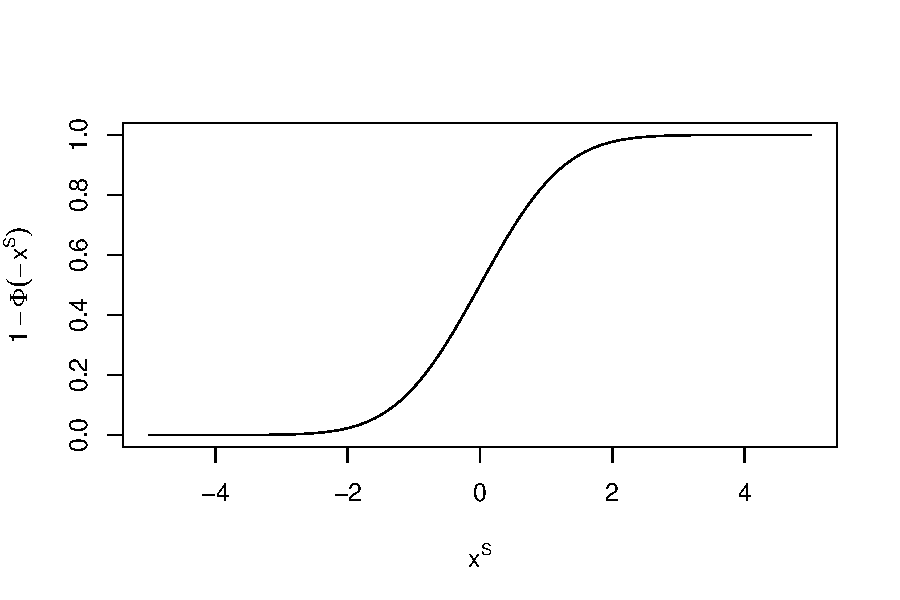
\includegraphics[width=\linewidth]{pnorm.pdf}
  \caption{Probability that $y^O$ is observable depending on the value
    of $x^S$ (given the standard normal disturbances).}
  \label{fig:pnorm}
\end{figure}





\section{Addtional notes}
\label{sec:additional}


In general, one should prefer \code{method="ml"} instead of
\code{"2step"}.  However, ML may have problems at the boundary of the
parameter space.  Consider the following problem: suppose we are
investigating the dependence of weight on individual characteristic
$x$.  However, our weight has an upper limit (say, $\bar w$).  Assume
the linear model and normal errors.  This creates the following
tobit-problem:
\begin{align}
  w_i^* &= \beta_0 + \beta x_i + \varepsilon_i\\
  w_i &=
  \begin{cases}
    w_i^* \quad & \text{if } w_i^* < \bar w\\
    \bar w      & \text{otherwise.}
  \end{cases}
\end{align}
The tobit model can be rewritten in the form of a tobit-2 equation
\begin{align}
  z_i^* &= \bar w_i - \beta_0 - \beta x_i - \varepsilon_i\\
  w_i^* &= \beta_0 + \beta x_i + \varepsilon_i\\
  z_i &=
  \begin{cases}
    1 \quad & \text{if } z_i^* > 0\\
    0       & \text{otherwise}
  \end{cases}\\
  w_i &=
  \begin{cases}
    w_i^* \quad & \text{if } w_i^* < \bar w\\
    \bar w      & \text{otherwise,}
  \end{cases}
\end{align}
where one can see, that the correlation of the error terms is $-1$.
In this case, the ML does not converge:
\begin{Code}
  x <- runif(500, -2, 2)
  e <- rnorm(500)
  z <- x + e > 0
  y <- (x - e)*z
  summary(selection(z ~ x, y ~ x, method="ml"))
\end{Code}
will give something like:
\begin{Code}
  Tobit 2 selection model/Maximum Likelihood estimation
  Newton-Raphson maximisation, 1 iterations
  Return code 3: Last step could not find a value above the current.
  May be near a solution
  Log-Likelihood: -984.8554 
  1000 observations (516 censored and 484 observed) and 6 free parameters (df =994)

  Probit selection equation:
  Estimate Std. error    t value      Pr(> t)
  (Intercept) -0.07032504 0.07274238 -0.9667685 3.336598e-01
  x            0.99332164 0.07956116 12.4850077 9.013464e-36

  OLS equation:
  Estimate Std. error t value Pr(> t)
  (Intercept) 0.3922726        NaN     NaN     NaN
  x           0.7454347        NaN     NaN     NaN

  Error terms data:
  Estimate Std. error   t value Pr(> t)
  sigma  1.185191        NaN       NaN     NaN
  rho   -0.999245 0.01348266 -74.11337       0
  --------------------------------------------
  Warning messages:
  1: Diagonal of variance-covariance matrix not positive!
  in: summary.maxLik(object, ...) 
  2: NaNs produced in: sqrt(hdiag) 
\end{Code}
while the two-step method works:
\begin{Code}
  summary(selection(z ~ x, y ~ x, method="2step"))
  Estimates:
  Estimate Std. Error t value  Pr(>|t|)    
  (Intercept) -0.34297    0.22213  -1.544    0.1232    
  x            1.17892    0.13976   8.435 3.517e-16 ***
  ---
  Signif. codes:  0 '***' 0.001 '**' 0.01 '*' 0.05 '.' 0.1 ' ' 1 
  Multiple R-Squared:0.7437,	Adjusted R-Squared:0.7427
  Residual correlation: -0.7143789, variance: 0.8260205
\end{Code}




\section{Conclusion}


%% Note: If there is markup in \(sub)section, then it has to be escape as above.

\bibliography{selection}
%\bibliography{/home/suapm095/Documents/Literatur/literatur}

\end{document}